\section{Introducción}
El propósito de este trabajo es hacer una reflexión acerca del calentamiento global, las consecuencias que este ha traído hasta el momento y lo que pasara en un futuro no muy lejano si no cambiamos nuestra forma de vivir el día a día. Hoy en día nos encontramos a una temperatura de $1^\circ$C mayor a la era preindustrial y se estima que esta aumenta a razón de $0.2^\circ$C cada 10 años

El pasado 6 de Octubre se presento Reporte del Panel Intergubernamental de Cambio Climático (IPCC) en el cual resaltan la importancia de reducir a la mitad nuestras emisiones de $CO_2$ en los próximos 10 si queremos salvar el planeta. En este reporte se hace énfasis de que el limite que existe para el aumento de temperatura es de $1.5^\circ$C aunque el escenario planteado no es nada amigable con esa temperatura, es mucho mejor y más prometedor que llegar a $2^\circ$C. Si bien $0.5^\circ$C no parece mucho, cuando hablamos de un aumento permanente a nivel mundial significará consecuencias enormes no solo a los ecosistemas naturales, si no también a la economía humana. \textcolor{blue}{"Limitar el calentamiento global a $1.5^\circ$C en comparación con $2^\circ$C reduciría los impactos desafiantes sobre los ecosistemas, la salud humana y el bienestar}, dijo Priyardarshi Shukla, Presidente del Centro Mundial para el Medio Ambiente y la Energía de la Universidad de Ahmedabad en la India y Autor del Informe Especial.

El secretario general de la ONU, Antonio Guterres emitió un comunicado en el que dijo que alcanzar esta meta requiere \textcolor{blue}{"una acción urgente y mucho más ambiciosa para reducir las emisiones a la mitad para 2030, y alcanzar las emisiones netas cero para 2050}.

\begin{figure}[H]
  \centering 
  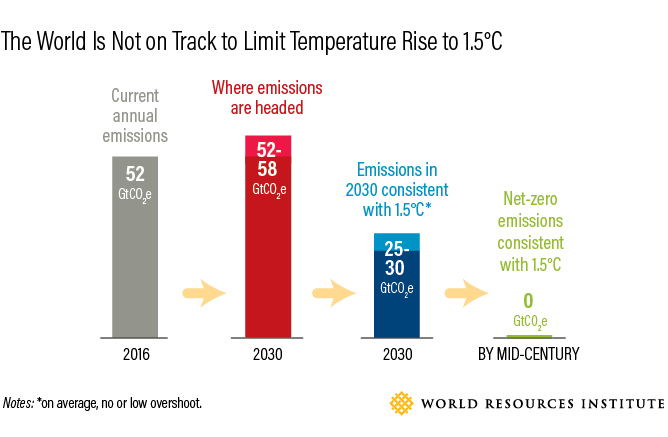
\includegraphics[width=0.32\textwidth]{figuras/grafica.png}
  \caption{Imagen de World Resources Institute}
  \label{fig:revista_inatel}
\end{figure}



